\chapter{HASIL YANG DIHARAPKAN}

\section{Hasil yang Diharapkan dari Penelitian}

\begin{figure} [ht] \centering
    % Nama dari file gambar yang diinputkan
    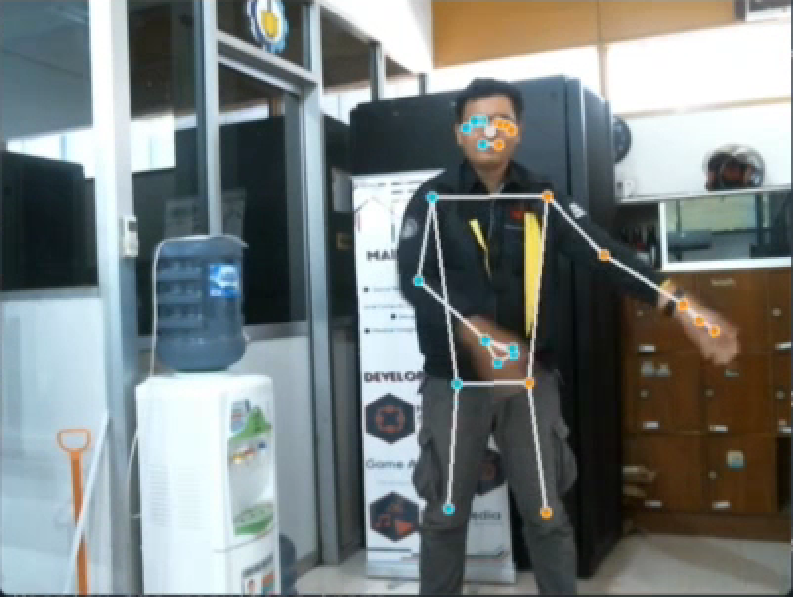
\includegraphics[scale=0.5]{gambar/contoh.png}
    % Keterangan gambar yang diinputkan
    \caption{Hasil Ujicoba Sementara Sejauh ini}
    % Label referensi dari gambar yang diinputkan
    \label{fig:Ujicoba Sementara}
  \end{figure}

Berdasarkan Hasil Ujicoba yang sudah dilakukan , Sejauh ini sudah terpasang software yang diperlukan seperti Jupyter Notebook , Anaconda , OpenCV , Python dan MediaPipe dan sudah melakukan program untuk memasang estimasi pose manusia yang berasal dari mediapipe dan juga sudah mulai bisa untuk melakukan pengambilan dataset
